\documentclass{standalone}
%\usepackage{showframe}
\usepackage{tikz}
\usetikzlibrary{shapes.arrows}

\begin{document}
\noindent
\begin{tikzpicture}
\begin{scope}
    \node[anchor=south west,inner sep=0] (image) at (0,0) {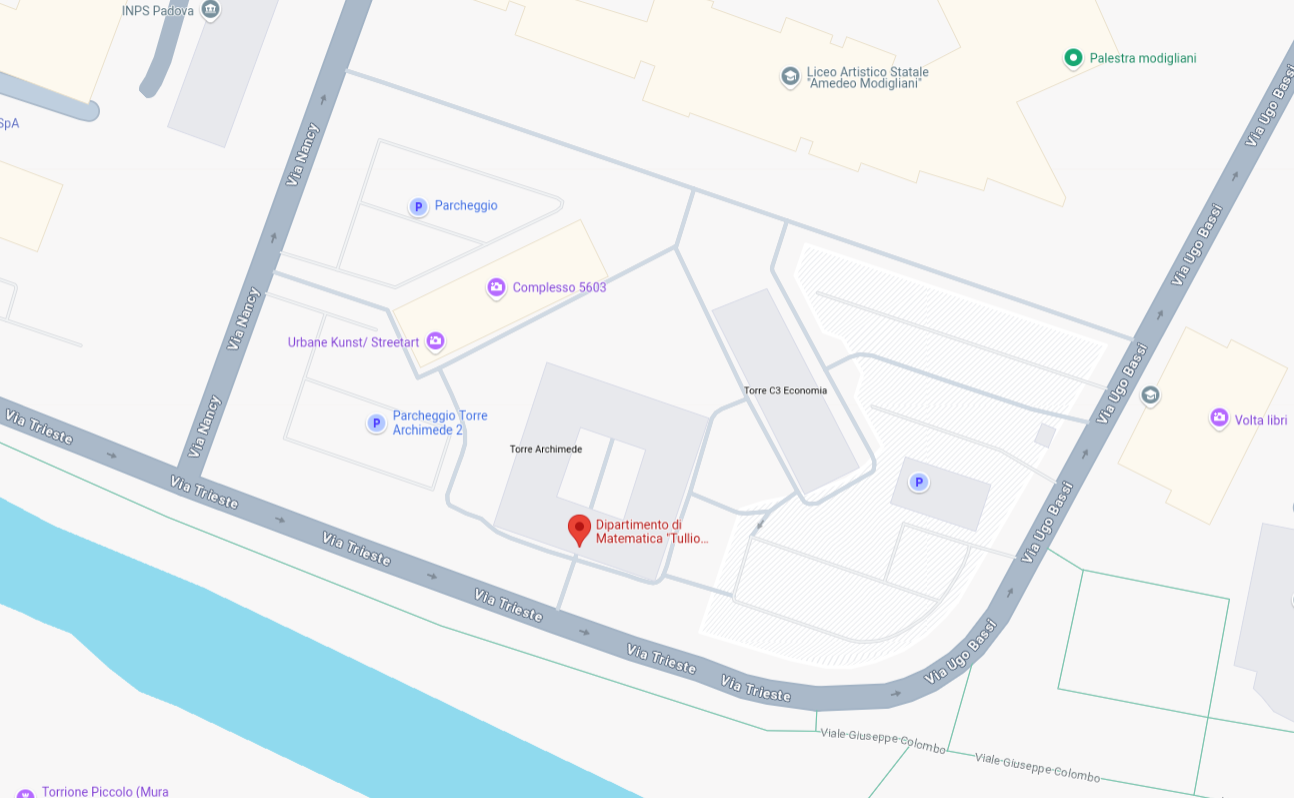
\includegraphics[width=\textwidth]{figures/google-maps-torre-archimede-3.png}};
    \coordinate (O) at (4.8,2.6);
    \draw[red, line width=3] (O) circle [radius=3mm];
    \node[fill=white, text=red] (T) at (3.8,1.2) {\Large\textbf{Entrance B}};
    \draw[->, >=latex, line width=2, red] ([yshift=1mm]T.north)
    .. controls (4,2) .. ([xshift=-4mm,yshift=-3mm]O);
\end{scope}
\end{tikzpicture}%
\end{document}
